%Este trabalho está licenciado sob a Licença Atribuição-CompartilhaIgual 4.0 Internacional Creative Commons. Para visualizar uma cópia desta licença, visite http://creativecommons.org/licenses/by-sa/4.0/deed.pt_BR ou mande uma carta para Creative Commons, PO Box 1866, Mountain View, CA 94042, USA.

\chapter{Perceptron}\label{cap_perceptron}
\thispagestyle{fancy}


\section{Unidade de Processamento}

A unidade básica de processamento (neurônio artificial) que exploramos nestas notas é baseado no \emph{perceptron} (consultemos a Fig. \ref{fig:perceptron}). Consiste na composição de uma \emph{função de ativação} $f:\mathbb{R}\to\mathbb{R}$ com a \emph{pré-ativação}
\begin{align}
  z &= \pmb{w}\cdot\pmb{x} + b\\
    &= w_1x_1 + w_2x_2 + \cdots + w_nx_n + b
\end{align}
onde, $\pmb{x}\in\mathbb{R}^{n}$ é o vetor de entrada, $\pmb{w}\in\mathbb{R}^{n}$ é o vetor de pesos e $b\in\mathbb{R}$ é o {\it bias}. Escolhida uma função de ativação, a saída do neurônio é dada por
\begin{align}
  y &:= \mathcal{N}\left(\pmb{x};(\pmb{w},b)\right)\\
    &= f(z) = f(\pmb{w}\cdot\pmb{x} + b)
\end{align}
O treinamento (calibração) consiste em determinar os parâmetros $(\pmb{w}, b)$ de forma que o neurônio forneça as saídas $y$ esperadas com base em algum critério predeterminado.

\begin{figure}[H]
  \centering
  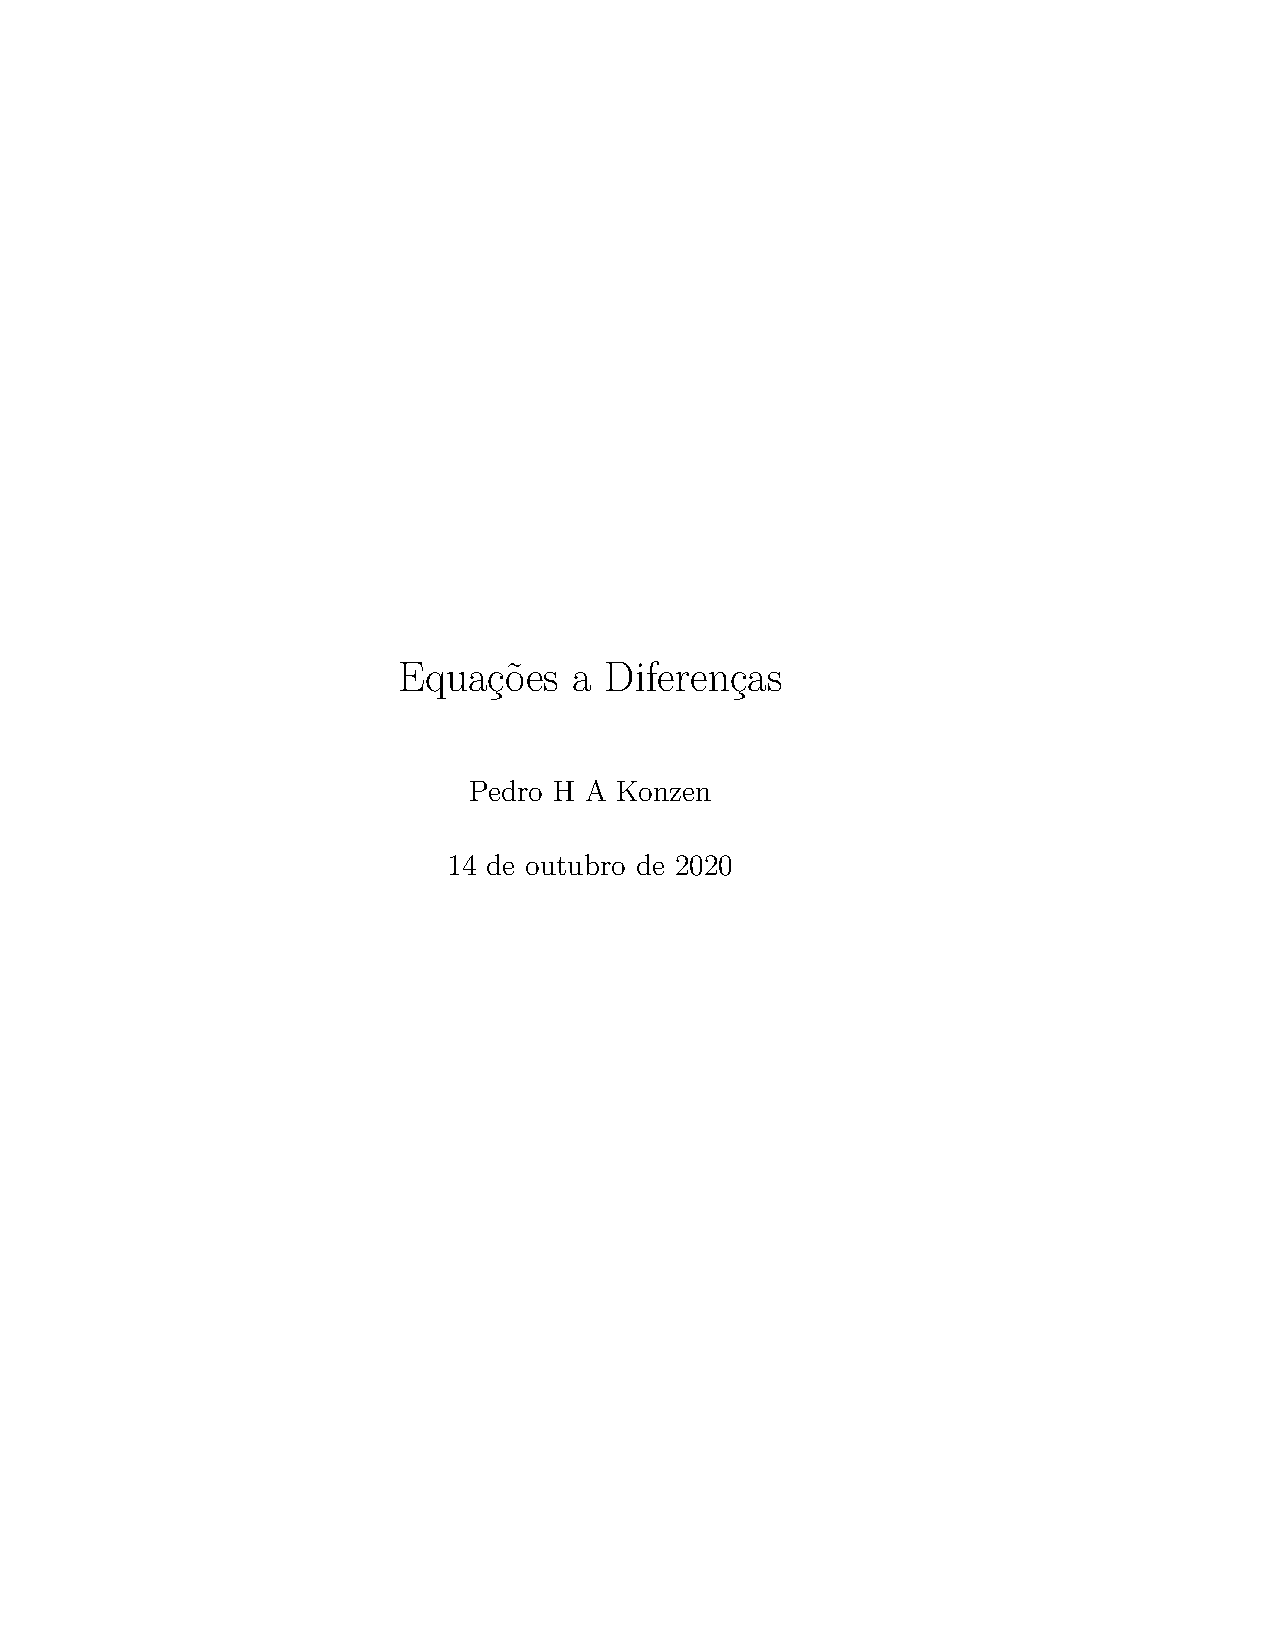
\includegraphics[width=0.7\textwidth]{./cap_perceptron/dados/neuronio/main}
  \caption{Esquema de um perceptron: unidade de processamento.}
  \label{fig:perceptron}
\end{figure}

Uma das vantagens deste modelo de neurônio é sua generalidade, i.e. pode ser aplicado a diferentes problemas. Na sequência, vamos aplicá-lo na resolução de um problema de classificação e noutro de regressão.


\subsection{Um problema de classificação}

Vamos desenvolver um perceptron que faça a operação $\land$ (e-lógico). I.e, receba como entrada dois valores lógicos $A_1$ e $A_2$ (V, verdadeiro ou F, falso) e forneça como saída o valor lógico $R = A_1 \land A_2$. Consultemos a seguinte tabela verdade:

\begin{center}
  \begin{tabular}{cc|c}
    $A_1$ & $A_2$ & R\\\hline
    V & V & V\\
    V & F & F\\
    F & V & F\\
    F & F & F\\\hline
  \end{tabular}
\end{center}


\subsubsection{Modelo}

Nosso modelo de neurônio será um perceptron com duas entradas $\pmb{x}\in \{-1,1\}^2$ e a função sinal
\begin{equation}
  f(z) = \sign(z) = \left\{
    \begin{array}{ll}
      1 &, z>0\\
      0 &, z=0\\
      -1 &, z<0
    \end{array}
\right.
\end{equation}
como função de ativação, i.e.
\begin{equation}
  \mathcal{N}\left(\pmb{x};(\pmb{w},b)\right) = \sign(\pmb{w}\cdot\pmb{x} + b),
\end{equation}
onde $\pmb{w}\in\mathbb{R}^2$ e $b\in\mathbb{R}$ são parâmetros a determinar.


\subsubsection{Pré-processamento}

Uma vez que nosso modelo recebe valores $\pmb{x}\in \{-1,1\}^2$ e retorna $y\in\{-1,1\}$, precisamos (pre)processar os dados do problema de forma a utilizá-lo. Uma forma, é assumir que todo valor negativo está associado ao valor lógico $F$ (falso) e positivo ao valor lógico $V$ (verdadeiro). Desta forma, os dados podem ser interpretados como na seguinte tabela

\begin{center}
  \begin{tabular}{rr|c}
    $x_1$ & $x_2$ & $y$\\\hline
    1 & 1 & 1\\
    1 & -1 & -1\\
    -1 & 1 & -1\\
    -1 & -1 & -1\\\hline
  \end{tabular}
\end{center}
    
    
\subsubsection{Treinamento}

Agora, nos falta treinar nosso neurônio para fornecer o valor de $y$ esperado para cada dada uma entrada $\pmb{x}$. Isso consiste em um método para escolhermos os parâmetros $(\pmb{w},b)$ que sejam adequados para esta tarefa. Vamos explorar mais sobre isso na sequência do texto e, aqui, apenas escolhemos
\begin{gather}
  \pmb{w} = (1, 1)\\
  b = -1
\end{gather}
Com isso, nosso perceptron é
\begin{equation}
  \mathcal{N}(\pmb{x}) = \sign(x_1 + x_2 - 1)
\end{equation}
Verifique que ele satisfaz a tabela verdade acima!


\subsubsection{Implementação}

\ifispython
Podemos implementar nosso perceptron usando {\python}+{\pytorch} como segue

\lstinputlisting{./cap_perceptron/dados/py_e/main.py}

Verifique! Aqui e nas seguintes implementações, utilizamos vários métodos para a manipulação de tensores \lstinline+torch.Tensor+). Consulte \href{https://pytorch.org/docs/stable/torch.html}{PyTorch Docs: torch} para mais informações sobre estes e muitos outros métodos disponíveis.
\fi

\subsubsection{Interpretação geométrica}

Empregamos o seguinte modelo de neurônio
\begin{equation}
  \mathcal{N}\left(\pmb{x};(\pmb{w},b)\right) = \sign(w_1x_1 + w_2x_2 + b)
\end{equation}
Observamos que
\begin{equation}
  w_1x_1 + w_2x_2 + b = 0
\end{equation}
corresponde à equação geral de uma reta no plano $\tau: x_1\times x_2$. Esta reta divide o plano em dois semiplanos
\begin{align}
  \tau^+ = \{\pmb{x}\in\mathbb{R}^2: w_1x_1 + w_2x_2 + b > 0\}\\
  \tau^- = \{\pmb{x}\in\mathbb{R}^2: w_1x_1 + w_2x_2 + b < 0\}
\end{align}
O primeiro está na direção do vetor normal a reta $\pmb{n} = (w_1, w_2)$ e o segundo na sua direção oposta. Com isso, o problema de treinar nosso neurônio para nosso problema de classificação consiste em encontrar a reta
\begin{equation}
  w_1x_1 + w_2x_2 + b = 0
\end{equation}
de forma que o ponto $(1,1)$ esteja no semiplano positivo $\tau^+$ e os demais pontos no semiplano negativo $\tau^-$. Consulte a Figura \ref{fig:class_e}.

\begin{figure}[H]
  \centering
  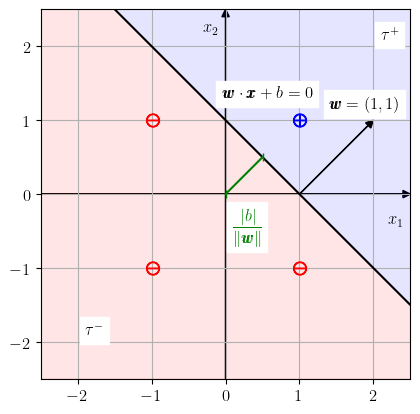
\includegraphics[width=0.7\textwidth]{./cap_perceptron/dados/fig_class_e/main}
  \caption{Interpretação geométrica do perceptron aplicado ao problema de classificação ralacionado à operação lógica $\land$ (e-lógico).}
  \label{fig:class_e}
\end{figure}

\subsubsection{Algoritmo de treinamento: perceptron}

O algoritmo de treinamento perceptron permite calibrar os pesos de um neurônio para fazer a classificação de dados linearmente separáveis. Trata-se de um algoritmo para o \emph{treinamento supervisionado} de um neurônio, i.e. a calibração dos pesos é feita com base em um dado \emph{conjunto de amostras de treinamento}.

Seja dado um \emph{conjunto de treinamento} $\{\pmb{x}^{(s)},y^{(s)}\}_{s=1}^{n_s}$, onde $n_s$ é o número de amostras. O algoritmo consiste no seguinte:
\begin{enumerate}
\item $\pmb{w} \leftarrow\pmb{0}$, $b \leftarrow 0$.
\item Para $e \leftarrow 1,\dotsc, n_e$:
  \begin{enumerate}
  \item Para $s \leftarrow 1,\dotsc, n_s$:
    \begin{enumerate}
    \item Se $y^{(s)}\mathcal{N}\left(\pmb{x}^{(s)}\right) \leq 0$:
      \begin{enumerate}
      \item $\pmb{w} \leftarrow \pmb{w}+y^{(s)}\pmb{x}^{(s)}$
      \item $b \leftarrow b + y^{(s)}$
      \end{enumerate}
    \end{enumerate}
  \end{enumerate}
\end{enumerate}
onde, $n_e$ é um dado número de épocas\footnote{Número de vezes que as amostrar serão percorridas para realizar a correção dos pesos.}.

\ifispython
Podemos implementar nosso algoritmo perceptron usando {\python}+{\pytorch} como segue

\lstinputlisting{./cap_perceptron/dados/py_percep_e/main.py}

Verifique!
\fi

\begin{teo}(Perceptron)
  \emconstrucao
\end{teo}

\subsection{Problema de regressão}

Vamos treinar um perceptron para resolver o problema de regressão linear para os seguintes dados

\begin{center}
  \begin{tabular}{l|ll}
    s & $x^{(s)}$ & $y^{(s)}$\\\hline
    1 & 0.5 & 1.2\\
    2 & 1.0 & 2.1\\
    3 & 1.5 & 2.6\\
    4 & 2.0 & 3.6\\\hline
  \end{tabular}
\end{center}

\subsubsection{Modelo}

Vamos determinar o perceptron\footnote{Escolhendo $f(z)=z$ como função de ativação.}
\begin{equation}\label{eq:percep_regr}
  \tilde{y} = \mathcal{N}(x; (w, b)) = wx + b
\end{equation}
que melhor se ajusta a este conjunto de dados $\left\{(x^{(s)}, y^{(s)})\right\}_{s=1}^{n_s}$, $n_s=4$.

\subsubsection{Treinamento}

A ideia é que o perceptron seja tal que minimize o erro quadrático médio (EQM)\footnote{Em inglês, \it{mean squared error} (MSE).}, i.e.
\begin{equation}\label{eq_percep:regr_prob}
  \min_{w,b}\frac{1}{n_s}\sum_{s=1}^{n_s}\left(\tilde{y}^{(s)}-y^{(s)}\right)^2
\end{equation}
Vamos denotar a \emph{função erro}\footnote{Em inglês, {\it loss function}.} por
\begin{align}\label{eq:eqm}
  \varepsilon(w,b) &:= \frac{1}{n_s}\sum_{s=1}^{n_s}\left(\tilde{y}^{(s)}-y^{(s)}\right)^2\\
                   &= \frac{1}{n_s}\sum_{s=1}^{n_s}\left(wx^{(s)}+b-y^{(s)}\right)^2
\end{align}

Observamos que \eqref{eq_percep:regr_prob} é equivalente a um problema linear de \href{https://notaspedrok.com.br/notas/MatematicaNumerica/cap_ajuste_sec_prob_lin.html}{mínimos quadrados}. A solução é obtida resolvendo-se a equação normal\footnote{Consulte o Exercício \ref{exer_percep:sol_mq}.}
\begin{equation}\label{eq_percep:sol_mq}
  M^TM\pmb{c} = M^T\pmb{y},
\end{equation}
onde $\pmb{c} = (w, p)$ é o vetor dos parâmetros a determinar e $M$ é a matriz $n_s\times 2$ dada por
\begin{equation}
  M =
  \begin{bmatrix}
    \pmb{x} & \pmb{1}
  \end{bmatrix}
\end{equation}

\subsubsection{Implementação}

\ifispython
Usando {\python}+{\pytorch}, podemos implementar nosso perceptron para o problema de regressão como segue

\lstinputlisting{./cap_perceptron/dados/py_percep_mq/main.py}

Verifique!
\fi

\subsubsection{Resultado}

Nosso perceptron corresponde ao modelo
\begin{equation}
  \mathcal{N}(x; (w,b)) = wx + b
\end{equation}
com os pesos treinados $w = 1.54$ e $b = 0.45$. Ele corresponde à reta que melhor se ajusta ao conjunto de dados de $\left\{x^{(s)}, y^{(s)}\right\}$. Consulte a Figura \ref{fig:percep_mq}.

\begin{figure}[H]
  \centering
  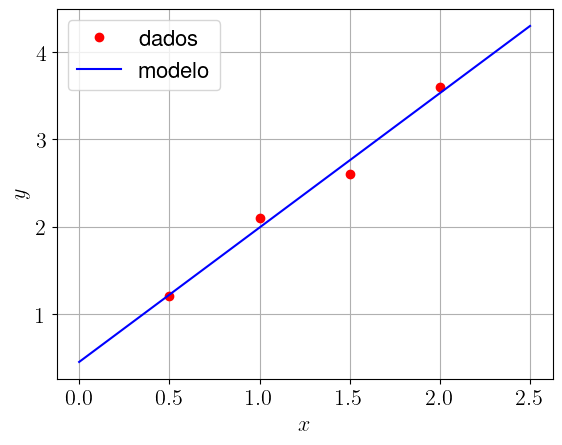
\includegraphics[width=0.7\textwidth]{./cap_perceptron/dados/fig_percep_mq/main}
  \caption{Interpretação geométrica do perceptron aplicado ao problema de regressão linear.}
  \label{fig:percep_mq}
\end{figure}

\subsection{Exercícios}

\begin{exer}\label{exer:eqm_convexa}
  Assumindo o modelo de neurônio \eqref{eq:percep_regr}, mostre que \eqref{eq:eqm} é função convexa.
\end{exer}
\begin{resp}
  Dica: verifique que sua matriz hessiana é positiva definida.
\end{resp}

\begin{exer}\label{exer_percep:sol_mq}
  Mostre que a solução do problema \eqref{eq_percep:regr_prob} é dada por \eqref{eq_percep:sol_mq}.
\end{exer}
\begin{resp}
  Dica: consulte a ligação \href{https://notaspedrok.com.br/notas/MatematicaNumerica/cap_ajuste_sec_prob_lin.html}{Notas de Aula: Matemática Numérica: 7.1 Problemas lineares}.
\end{resp}

\emconstrucao

\section{Algoritmo de Treinamento}

Na seção anterior, desenvolvemos dois modelos de neurônios para problemas diferentes, um de classificação e outro de regressão. Em cada caso, utilizamos algoritmos de treinamento diferentes. Agora, vamos estudar algoritmos de treinamentos mais gerais\footnote{Aqui, vamos explorar apenas algoritmos de treinamento supervisionado.}, que podem ser aplicados a ambos os problemas.

Ao longo da seção, vamos considerar o modelo de neurônio
\begin{equation}
  \mathcal{N}\left(\pmb{x}; (\pmb{w}, b)\right) = f(\pmb{w}\cdot\pmb{x} + b),
\end{equation}
com dada função de ativação $f:\mathbb{R}\to\mathbb{R}$, sendo os vetores de entrada $\pmb{x}$ e dos pesos $\pmb{w}$ de tamanho $n_{in}$. A pré-ativação do neurônio é denotada por
\begin{equation}
  z := \pmb{w}\cdot\pmb{x} + b
\end{equation}

Fornecido um conjunto de treinamento $\left\{\left(\pmb{x}^{(s)}, y^{(s)}\right)\right\}_1^{n_s}$, com $n_s$ amostras, o objetivo é calcular os parâmetros $(\pmb{w}, b)$ que minimizam a função erro quadrático médio
\begin{align}\label{eq:percep_mse}
  \varepsilon(\pmb{w}, b) &:= \frac{1}{n_s}\sum_{s=1}^{n_s}\left(\tilde{y}^{(s)} - y^{(s)}\right)^2\\
                          &= \frac{1}{n_s}\sum_{s=1}^{n_s}\varepsilon^{(s)}
\end{align}
onde $\tilde{y}^{(s)} = \mathcal{N}\left(\pmb{x}^{(s)}; (\pmb{w}, b)\right)$ é o valor estimado pelo modelo para a $s$-ésima amostra e $\varepsilon^{(s)} := \left(\tilde{y}^{(s)} - y^{(s)}\right)^2$. I.e., queremos resolver o seguinte problema de otimização
\begin{equation}
  \min_{(\pmb{w}, b)}\varepsilon(\pmb{w}, b)
\end{equation}

Para resolver este problema de otimização, vamos empregar o Método do Gradiente Descendente. Como veremos na sequência, ele requer o cálculo de derivadas da função erro e da função de ativação. Por isso, antes de o estudarmos, vamos fazer uma implementação mais detalhada de nosso modelo, da função erro e da função de ativação. A ideia é termos um código mais adequado e que nos dê acesso fácil as derivadas necessárias para o algoritmo de treinamento.

\subsubsection{Função de Ativação}

Por simplicidade, vamos assumir a função identidade como função de ativação, i.e. $f(z)=z$. A implementamos com o seguinte código:

\ifispython
\lstinputlisting[firstline=3, lastline=12]{./cap_perceptron/dados/py_gd/main.py}
\fi

Aqui, a classe \lstinline+IdentityFun+ implementa a função identidade com dois métodos. O método \lstinline+value+ retorna o valor da função para uma dada entrada $z$, i.e. computa $f(z)$. O método \lstinline+grad+ computa a derivada da função, i.e. $f'(z)$.

\subsubsection{Unidade de Processamento}

Nosso modelo consiste em apenas uma unidade de processamento do tipo perceptron. O seguinte código implementa-o como uma classe.

\ifispython
\lstinputlisting[firstline=14, lastline=33]{./cap_perceptron/dados/py_gd/main.py}
\fi

A classe contém o método \lstinline+forward+ que computa a saída do modelo para uma dada entrada $\pmb{x}$, i.e., calcula
\begin{equation}
  y = \mathcal{N}\left(\pmb{x}; (\pmb{w}, b)\right).
\end{equation}

\subsubsection{Função Erro}

Nossa função erro\footnote{Em inglês, {\it loss function}.} é dada em \eqref{eq:percep_mse}. A implementamos como a seguinte classe.

\ifispython
\lstinputlisting[firstline=35, lastline=51]{./cap_perceptron/dados/py_gd/main.py}
\fi

Nela o método \lstinline+partial+ computa $\varepsilon^{(s)} = \left(\tilde{y}^{(s)}-y^{(s)}\right)^2$ e o método \lstinline+grad+ computa a seguinte derivada
\begin{equation}
  \frac{\p\varepsilon^{(s)}}{\p \tilde{y}^{(s)}} = 2\left(\tilde{y}^{(s)}-y^{(s)}\right)
\end{equation}

\subsection{Método do Gradiente Descendente}

O Método do Gradiente Descendente\footnote{Em inglês, {\it Gradiente Descent, GD Method}.} (GD) é um \href{https://notaspedrok.com.br/notas/MatematicaNumericaAvancada/cap_otimizacao_sec_minimi.html}{método de declive}. Aplicado ao nosso modelo de perceptron consiste no seguinte algoritmo:
\begin{enumerate}
\item $\pmb{w}, b$ aproximações iniciais.
\item Para $e\leftarrow 1, \dotsc, n_e$:
  \begin{enumerate}
  \item $\displaystyle (\pmb{w}, b) \leftarrow (\pmb{w}, b) - l_r\frac{\p\varepsilon}{\p (\pmb{w}, b)}$
  \end{enumerate}
\end{enumerate}
onde, $n_e$ é o \emph{número de épocas}, $l_r$ é uma dada \emph{taxa de aprendizagem}\footnote{Em inglês, {\it learning rate}.} e o gradiente é
\begin{equation}
  \frac{\p\varepsilon}{\p (\pmb{w}, b)} := \left(\frac{\p\varepsilon}{\p w_1}, \dotsc, \frac{\p\varepsilon}{\p w_{n_{in}}}, \frac{\p\varepsilon}{\p b}\right)
\end{equation}

O cálculo do gradiente para os pesos $\pmb{w}$ pode ser feito como segue
\begin{align}
  \frac{\p\varepsilon}{\p \pmb{w}} &= \frac{\p}{\p\pmb{w}}\left[\frac{1}{n_s}\sum_{s=1}^{n_s}\varepsilon^{(s)}\right]\\
                                   &= \frac{1}{ns}\sum_{s=1}^{ns}\frac{\p\varepsilon^{(s)}}{\p\tilde{y}^{(s)}}\frac{\p\tilde{y}^{(s)}}{\p\pmb{w}}\\
  {\color{blue}\frac{\p\varepsilon}{\p \pmb{w}}} &{\color{blue}= \frac{1}{ns}\sum_{s=1}^{ns}\frac{\p\varepsilon^{(s)}}{\p\tilde{y}^{(s)}}\frac{\p\tilde{y}^{(s)}}{\p z^{(s)}}\frac{\p z^{(s)}}{\p\pmb{w}}}\\
\end{align}
Observando que
\begin{gather}
  \frac{\p\varepsilon^{(s)}}{\p\tilde{y}^{(s)}} = 2\left(\tilde{y}^{(s)} - y^{(s)}\right)\\
  \frac{\p\tilde{y}^{(s)}}{\p z^{(s)}} = f'\left(z^{(s)}\right)\\
  \frac{\p z^{(s)}}{\p\pmb{w}} = \pmb{x}^{(s)}
\end{gather}
obtemos
\begin{equation}
  \frac{\p\varepsilon}{\p \pmb{w}} = \frac{1}{n_s}\sum_{s=1}^{n_s}2\left(\tilde{y}^{(s)}-y^{(s)}\right)f'\left(z^{(s)}\right)\pmb{x}^{(s)}
\end{equation}
\begin{align}
  {\color{blue}\frac{\p\varepsilon}{\p b}} &{\color{blue}= \frac{1}{ns}\sum_{s=1}^{ns}\frac{\p\varepsilon^{(s)}}{\p\tilde{y}^{(s)}}\frac{\p\tilde{y}^{(s)}}{\p z^{(s)}}\frac{\p z^{(s)}}{\p b}}\\
  \frac{\p\varepsilon}{\p b} &= \frac{1}{n_s}\sum_{s=1}^{n_s}2\left(\tilde{y}^{(s)}-y^{(s)}\right)f'\left(z^{(s)}\right)\cdot 1
\end{align}

\emconstrucao

\subsection{Exercícios}

\emconstrucao

